%Template credit: Jan-Willem Steeb, NRAO

\documentclass[12pt,a4paper]{article}

\usepackage{graphics,graphicx}
\usepackage[%
    font={small,sf},
    labelfont=bf,
    format=hang,    
    format=plain,
    margin=0pt,
    width=0.8\textwidth,
]{caption}
\usepackage[list=true]{subcaption}
\usepackage{amsmath}
\usepackage{amssymb}
\usepackage{bm}
\usepackage{listings}
\usepackage{hyperref}
\usepackage{lmodern}  
\usepackage{amsmath}  
\usepackage{xcolor}   
\lstset{
  basicstyle=\ttfamily,
  columns=fullflexible,
  frame=single,
  breaklines=true,
  postbreak=\mbox{\textcolor{red}{$\hookrightarrow$}\space},
}

\textheight=247mm
\textwidth=180mm
\topmargin=-7mm
\oddsidemargin=-10mm
\evensidemargin=-10mm
\parindent 10pt

%%%%%%%%%%%%%%%%%%%%%
%%%%% Custom Commands %%%%
%%%%%%%%%%%%%%%%%%%%%
\newcommand{\vb}[1]{\text{\textbf{#1}}} %make non special characters bold in math mode, used for vectors and matrices
\newcommand{\n}[1]{\text{{#1}}} %removes math styling, useful for subscripts

%Mathematic Functions
\DeclareMathOperator*{\argmax}{arg\,max}
\DeclareMathOperator*{\argmin}{arg\,min}
\DeclareMathOperator*{\mmid}{mid}
\DeclareMathOperator*{\at}{arctan2}

%%%%%%%%%%%%%%%%%%%%%
%%%%% Start of document %%%%% 
%%%%%%%%%%%%%%%%%%%%%

\begin{document}
\pagestyle{plain}
\pagenumbering{arabic}
 
%%%%%%%%%%%%%
%%%%% Title  %%%%%
%%%%%%%%%%%%%%

\begin{center}
{\Large{\bf{  Data Comb 2019 Memo template \\  }}} 

\end{center}
\bigskip

\centerline{Author Name (Institution); Author Name (Institution); Author Name (Institution); etc.}

\centerline{\today}
\bigskip

%%%%%%%%%%%%%%%%%%%%%%%%%%%
%% Please include this line
\noindent \textit{This memo was prepared as part of the workshop ``Improving Image Fidelity on Astronomical Data: Radio Interferometer and Single-Dish Data Combination,'' held on 12-16 Aug 2019 at the Lorentz Center in Leiden, The Netherlands.}
%%%%%%%%%%%%%%%%%%%%%%%%%%%

\section{Dataset overview}

%% Begin your text here.
\textbf{One memo per group, please.} Describe the dataset (observations or simulation) here.  You may include several important observing parameters in Table \ref{fig:aboutdata}.


%% You may edit this as you like; add/omit parameters; improve the format; etc. for your needs.
\begin{table}[!hbt]
\caption{Observational details (edit as needed)}\label{fig:aboutdata}              % title of Table
\label{table:1}      % is used to refer this table in the text
\centering                                      % used for centering table
\begin{tabular}{l c }          % centered columns (4 columns)
\hline\hline                        % inserts double horizontal lines
Parameter & Value  \\    % table heading
\hline                                   % inserts single horizontal line
Phase center & J2000 16h09m18.1 -39d04m44.0 \\      % inserting body of the table
Rest frequency & 115.27120GHz \\
$V_{LSR}$ & 4 km/s \\
$\Delta V$ (channel width) & 1 km/s \\
Velocity range imaged & [5-8] km/s \\
Map size & NN $\times$ NN $^{\prime\prime}$\\
12m-array pointings & 29\\
7m-array pointings & 11\\
12m-array beamsize & NN $\times$ NN $^{\prime\prime}$ (PA=NN$^{\circ}$)\\
7m-array beamsize & NN $\times$ NN $^{\prime\prime}$ (PA=NN$^{\circ}$)\\
Range of 12m baselines & [15 - 453] m\\
Range of 7m baselines & [9 - 49] m\\
\hline                                             %inserts single line
\end{tabular}
\end{table}


\begin{figure}[!htb]
\centering
\subcaptionbox{For example, a plot of the mosaic pointings. \label{fig:1}}{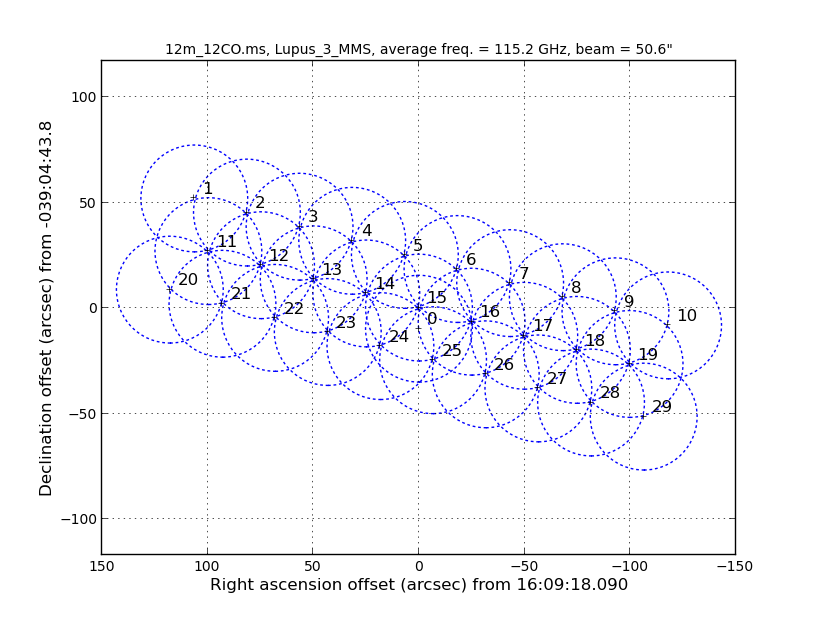
\includegraphics[width=0.49\textwidth]{images/12m_mosaic.png}}
\hfill
\subcaptionbox{Some weights. \label{fig:2}}{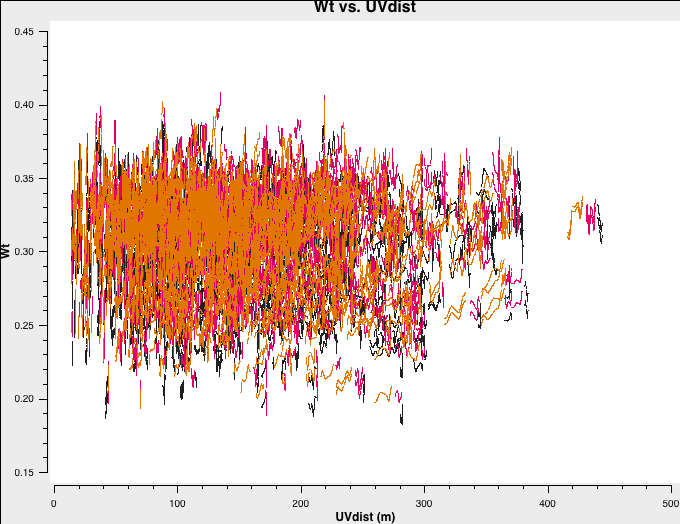
\includegraphics[width=0.49\textwidth]{images/12m_WT.png}}%
\hfill
\vspace{20pt}
\caption{\label{fig:example}}
\end{figure}

\section{Combination Methods}

\subsection{Method 1: Feather}

\subsection{Method 2: Joint Deconvolution (tp2vis)}

\subsection{Method 3 (If applicable): Specify}

\section{Comparison and evaluation}

In this section, you present the thorough (and challenging) work to both qualitatively \textbf{and quantitatively} compare the methods, and evaluate which one works better/best in the case of the dataset you tested.  \textbf{These methods are not directly provided to you.  Instead, you should develop in your group the methods to evaluate the ``goodness'' of each combination.}

Be as specific as possible.  If you know *why* one method worked differently than another, if you can include equations, snippets of code (here, or in Appendix below), or plots of quantitative metrics, then we can deeply understand and tackle the sometimes subtle differences in the methods.  Ideally, these code snippets will be useful to users in the future when they publish combined data, in order to assess the outcome.  

\subsection{ Equations, if needed}

Example equation:
\begin{align}
\vb{I}_{\n{tar},\epsilon} &=  \underbrace{\left\lbrace \kappa \bm{\delta} + \frac{1-\kappa}{ r_\Omega} ~~\mathcal{F}^{-1} \left( \frac{\vb{D}^f_{\n{psf}}}{\vb{B}^f_{\n{psf}}} \right) \right\rbrace}_{\vb{E}_1} * \vb{B}_{\n{tar}} * \vb{I}_{\n{signal}} + \underbrace{ \left\lbrace \frac{1}{r_\Omega}  ~~\mathcal{F}^{-1}  \left(\frac{\vb{D}^f_{\n{psf}}}{\vb{B}^f_{\n{psf}}} \right) \right\rbrace}_{\vb{E}_2}  * \vb{B}_{\n{tar}} * \vb{I}_{\n{noise}}, \label{eq:example}
\end{align}

Some pointers when writing equations using equation~\ref{eq:example} as an example:
\begin{itemize}
\item Matrices are indicated by  bold upper-case letters using \texttt{\textbackslash vb\{\}} (vectors are bold lower-case letters). 
\item When Greek letters should be bold use  \texttt{\textbackslash bm\{\}}. 
\item Math mode font can be removed using \texttt{\textbackslash n\{\}}. This is useful when subscripts or superscript text is not an index but a descriptor. For example, $\vb{I}_{\n{psf}}$ the subscript psf stands for point spread function.
\item Fancy letters to represent transforms (such as the Fourier transform $\mathcal{F}$) or number sets (choose one style  and be consistent) :
\begin{align*}
RQSZ \\
\mathcal{RQSZ} \\
\mathfrak{RQSZ} \\
\mathbb{RQSZ}
\end{align*}
\end{itemize}

%Tagging of equations
%Underlining equations

\subsection{Just a note about adding Images}

In figure~\ref{fig:example} multiple images are displayed using \texttt{\textbackslash subcaptionbox\{\}}. Any number of images can be displayed. A new row is created each time the sum of width parapeters is greater then \texttt{1\textbackslash textwidth}.  Of course, you can use your favorite method to include figures.

\begin{figure}[!htb]
\centering
{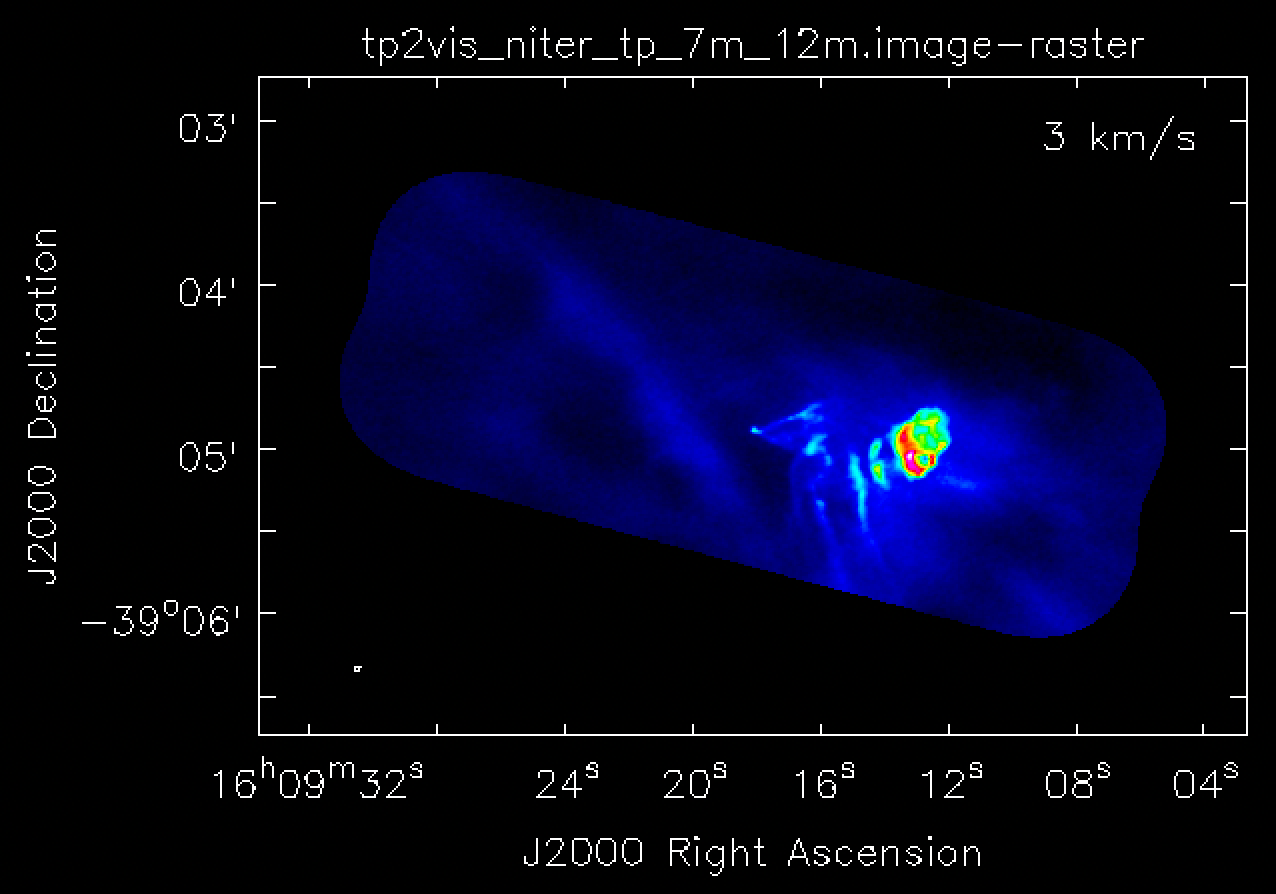
\includegraphics[width=0.49\textwidth]{images/tp2vis_3kms.png}}
\hfill
\caption{\label{fig:example}}
\end{figure}

\section{Additional notes, comments, challenges encountered}

Organize as you wish.  Please, if you discovered an issue during this workshop, document it as an issue in the Github.  

\clearpage
\section{Appendix: Code}

\begin{lstlisting}[language=Python]
def gauss_beam_abg(amp,parms_abg,x,y):
    a = parms_abg[0]
    b = parms_abg[1]
    g = parms_abg[2]
    r = a*(x**2) + b*x*y + g*y**2
    B = amp*np.exp(-r)
    return B
\end{lstlisting}



\end{document}